%!TEX program = xelatex
% 完整编译: xelatex -> bibtex -> xelatex -> xelatex
\documentclass[lang=cn,11pt,a4paper,cite=authoryear]{elegantpaper}




% 本文档命令
\usepackage{array}
\usepackage[final]{pdfpages}
\usepackage{graphicx}
\usepackage{float}
\newcommand{\ccr}[1]{\makecell{{\color{#1}\rule{1cm}{1cm}}}}

\begin{document}

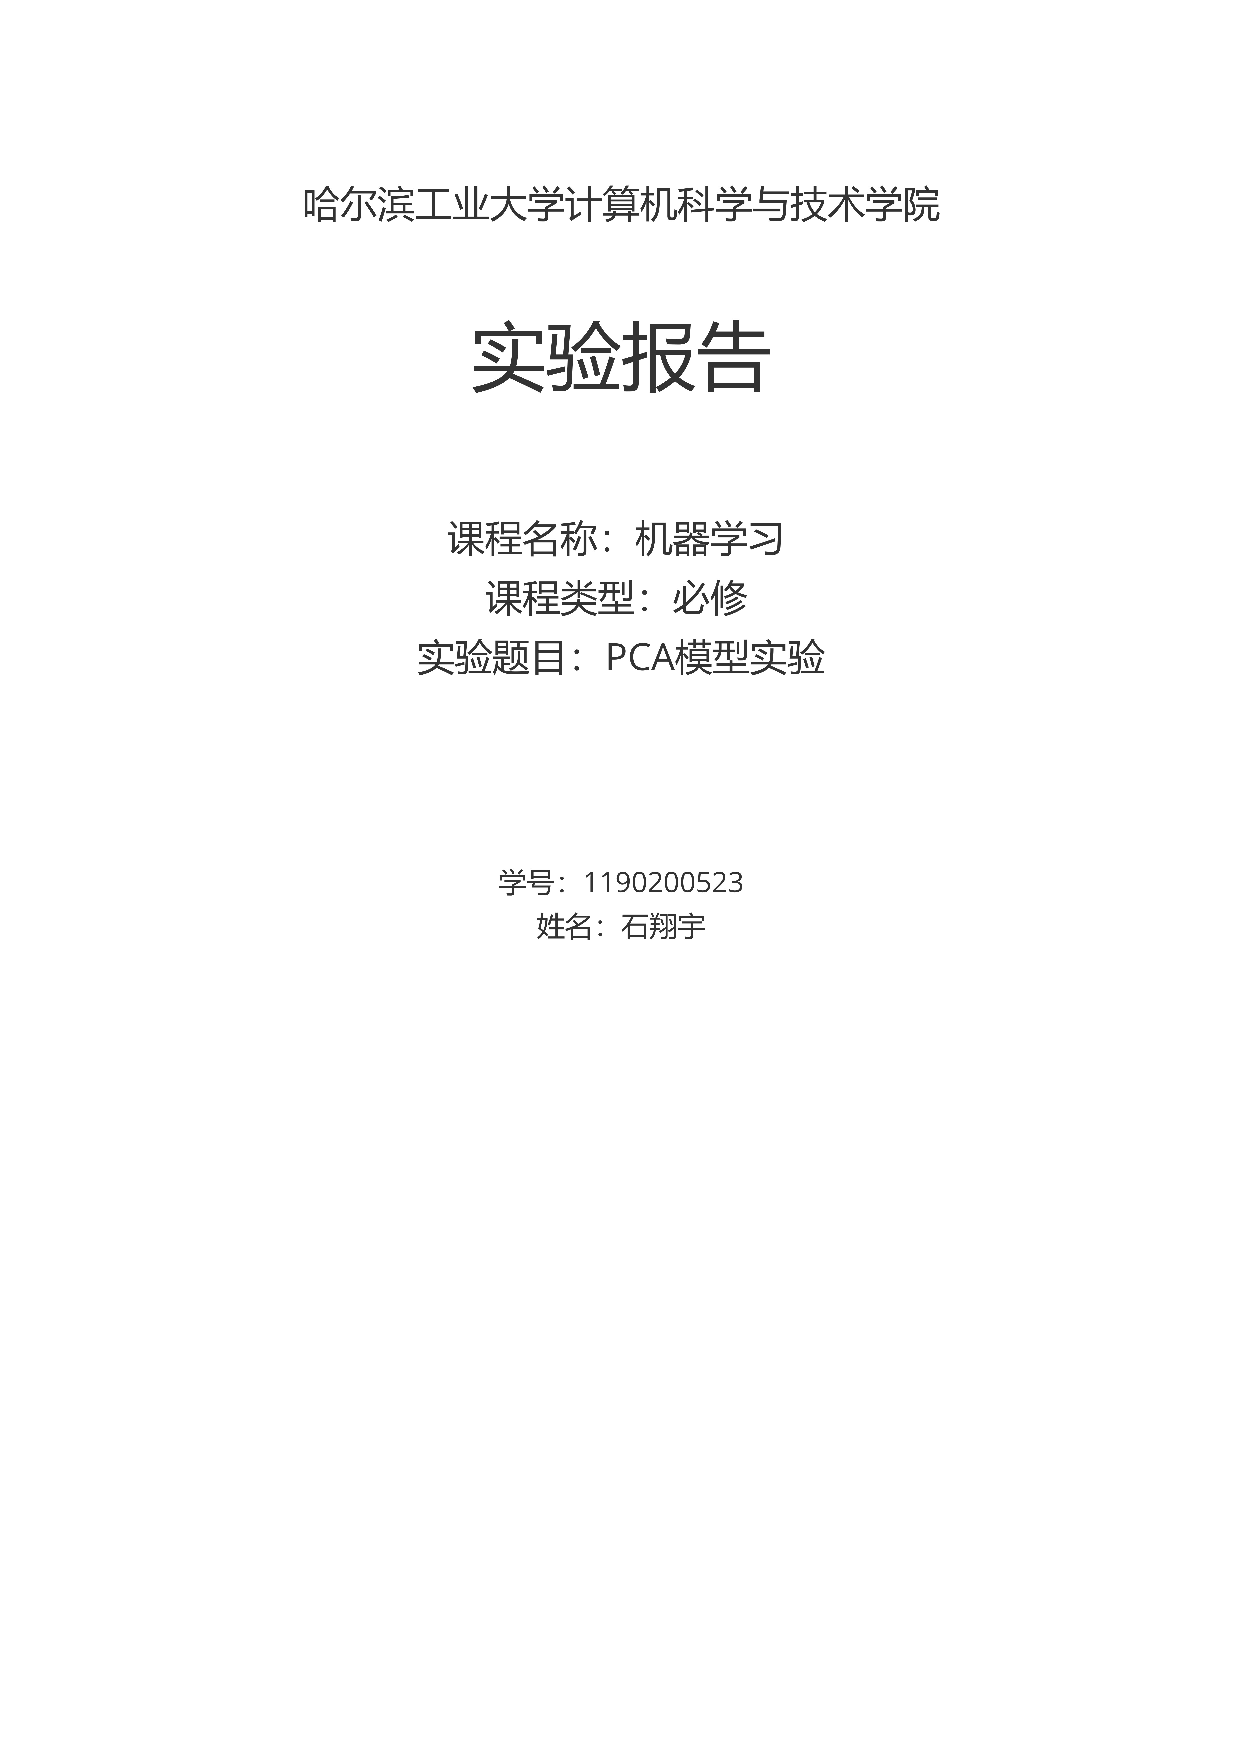
\includepdf{images/cover.pdf} 
\newpage

\section{实验目的}

实现一个PCA模型,能够对给定数据进行降维(即找到其中的主成分)。

\section{实验要求及实验环境}

\subsection{实验要求}

\paragraph{测试}


\begin{enumerate}
	\item 人工生成一些数据(如三维数据),让它们主要分布在低维空间中,如首先让某个维度的方差远小于其它唯独,然后对这些数据旋转。生成这些数据后,用你的PCA方法进行主成分提取;
	\item 找一个人脸数据(小点样本量),用你实现PCA方法对该数据降维,找出一些主成分,然后用这些主成分对每一副人脸图像进行重建,比较一些它们与原图像有多大差别(用信噪比衡量)。
\end{enumerate}

\subsection{实验环境}

Windows 11 + Python 3.7.8

\section{设计思想}

主成分分析(PCA)是一种常用的无监督学习方法,利用正交变换把线性相关变量表示的观测数据转换为少数几个由线性无关变量表示的数据,线性无关的变量称为主成分。

假设$X=(x_1,x_2,\dots,x_m)^T$是$m$维随机变量,其均值向量是
\begin{equation}
\mu=E(x)=(\mu_1,\mu_2,\dots,\mu_m)^T
\end{equation}
协方差矩阵是
\begin{equation}
\Sigma=cov(X,X)=E[(X-\mu)(x-\mu)^T]
\end{equation}
考虑由$m$维随机变量$X$到$m$维随机变量$Y=(y_1,y_2,\dots,y_m)^T$的线性变换
\begin{equation}
y_i=\alpha_i^TX=\alpha_{1i}x_1+\alpha_{2i}x_2+\dots+\alpha_{mi}x_m
\label{eq:1}
\end{equation}
其中$\alpha_i^T=(\alpha_{1i},\alpha_{2i},\dots,\alpha_{mi}),i=1,2,\dots,m$。

由随机变量的性质可知
\begin{align}
	&E(y_i)=\alpha_i^T\mu, \quad i=1, 2, \dots,m\\
	&var(y_i)=\alpha_i^T\Sigma\alpha_i, \quad i=1, 2, \dots,m\\
	&cov(y_i,y_j)=\alpha_i^T\Sigma\alpha_j, \quad i=1, 2, \dots,m\\
\end{align}
若如式\ref{eq:1}所示的线性变换满足下列条件

\begin{enumerate}
\item 系数变量$\alpha_i^T$是单位向量,即$\alpha_i^T\alpha_i=1, i=1,2,\dots,m$;
\item 变量$y_i$与$y_j$互不相关,即$cov(y_i,y_j)=0(i\not=j)$;
\item $y_i$是与$y_1,y_2,\dots,y_{i-1}\ (i=1, 2,\dots,m)$都不相关的$X$的所有线性变换中方差最大的,这时分别称$y_1,y_2,\dots,y_m$为$X$的第一主成分、第二主成分、…、第$m$主成分。
\end{enumerate}
	
我们将采用拉格朗日乘子法求出主成分。

首先求$X$的第一主成分$y_1=\alpha_1^TX$,即求系数向量$\alpha_1$。由主成分需要满足的条件可知,第一主成分的$\alpha_1$是在$\alpha_1^T\alpha_1=1$的条件下,$X$的所有线性变换中使方差
\begin{equation}
var(\alpha_1^TX)=\alpha_1^T\Sigma\alpha_1
\end{equation}
达到最大的。

求解第一主成分就是求解优化问题
\begin{equation}
\max_{\alpha_1}\ \alpha_1^T\Sigma\alpha_1\\
s.t.\ \alpha_1^T\alpha_1=1
\end{equation}
定义拉格朗日函数
\begin{equation}
L_1=\alpha_1^T\Sigma\alpha_1-\lambda(\alpha_1^T\alpha_1-1)
\end{equation}
其中$\lambda$是拉格朗日乘子。将$L_1$对$\alpha_1$求导,并令导数为$0$,得
\begin{equation}
\begin{aligned}
	\frac{\partial L_1}{\partial \alpha_1}=&2\Sigma\alpha_1-2\lambda\alpha_1=0
\end{aligned}
\end{equation}
因此,$\lambda$是$\Sigma$的特征值,$\alpha_1$是对应的单位特征向量,
\begin{equation}
L_1 =\alpha_1^T\Sigma\alpha_1-\lambda(\alpha_1^T\alpha_1-1)=\alpha_1^T\Sigma\alpha_1-\lambda\alpha_1^T\alpha_1+\lambda= \lambda
\end{equation}
假设$\Sigma$的最大特征值$\lambda_1$对应单位特征向量$\alpha_1$,则$\lambda_1$和$\alpha_1$是最优化问题的解
\begin{equation}
var(\alpha_1^TX)=\alpha_1^T\Sigma\alpha_1=\lambda_1
\end{equation}
求解第二主成分需要求解约束最优化问题
\begin{equation}
\max_{\alpha_2}\ \alpha_2^T\Sigma\alpha_2\\
s.t.\ \alpha_2^T\alpha_2=1, \quad \alpha_1^T\Sigma\alpha_2=0, \quad \alpha_2^T\Sigma\alpha_1=0
\end{equation}
注意到
\begin{equation}
\alpha_2^T\Sigma\alpha_1=\alpha_1^T\Sigma\alpha_2=\lambda_1\alpha_2^T\alpha_1=\lambda_1\alpha_1^T\alpha_2=0
\end{equation}
则定义拉格朗日函数
\begin{equation}
L_2=\alpha_2^T\Sigma\alpha_2-\lambda(\alpha_2^T\alpha_2-1)-\phi\alpha_2^T\alpha_1
\end{equation}
其中,$\lambda$和$\phi$是拉格朗日乘子。将$L_2$对$\alpha_2$求导,并令导数为$0$,得
\begin{equation}
\begin{aligned}
	\frac{\partial L_2}{\partial \alpha_1}=2\Sigma\alpha_2-2\lambda\alpha_2-\phi\alpha_1=&0\\
	2\alpha_1^T\Sigma\alpha_2-2\alpha_1^T\lambda\alpha_2-\alpha_1^T\phi\alpha_1=&0\\
	\phi\alpha_1^T\alpha_1=&0\\
	\phi=&0\\
	\\
	\Sigma\alpha_2-\lambda\alpha_2=&0\\
\end{aligned}
\end{equation}
由此,$\lambda$是$\Sigma$的特征值,$\alpha_2$是对应的单位特征向量,
\begin{equation}
\begin{aligned}
	L_2=&\alpha_2^T\Sigma\alpha_2-\lambda(\alpha_2^T\alpha_2-1)-\phi\alpha_2^T\alpha_1\\
	=&\alpha_2^T\Sigma\alpha_2-\lambda\alpha_2^T\alpha_2+\lambda\\
	=&\lambda\\
\end{aligned}
\end{equation}
假设$\Sigma$的第二大特征值$\lambda_2$对应单位特征向量$\alpha_2$,则$\lambda_2$和$\alpha_2$是最优化问题的解
\begin{equation}
var(\alpha_2^TX)=\alpha_2^T\Sigma\alpha_2=\lambda_2
\end{equation}
按照上述放大求得第一、第二、直到第$m$主成分,其系数向量$\alpha_1,\alpha_2,\dots,\alpha_m$分别是$\Sigma$的第一个、第二个、直到第$m$个单位特征向量,$\lambda_1,\lambda_2,\dots,\lambda_m$分别是对应的特征值。

\section{实验结果分析}

\subsection{人工数据测试}
我们生成了“瑞士卷”数据。“瑞士卷”数据是分布在三维空间的瑞士卷结构,正投影为漩涡状。我们设定数据量为$2000$,噪声系数为$0.1$,生成的数据如\figref{fig:mllab41}所示。

\begin{figure}[H]
	\centering
	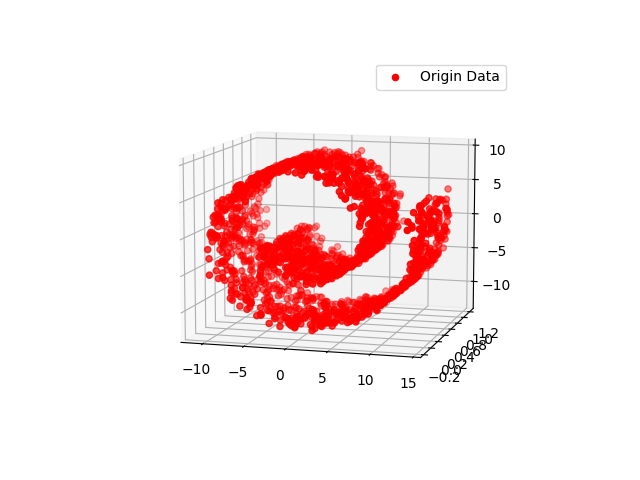
\includegraphics[width=0.7\linewidth]{images/ml_lab4_1.png}
	\caption{}
	\label{fig:mllab41}
\end{figure}

我们使用PCA算法将三维的“瑞士卷”结构降维到二维空间中,结果如\figref{fig:mllab42}所示。

\begin{figure}[H]
	\centering
	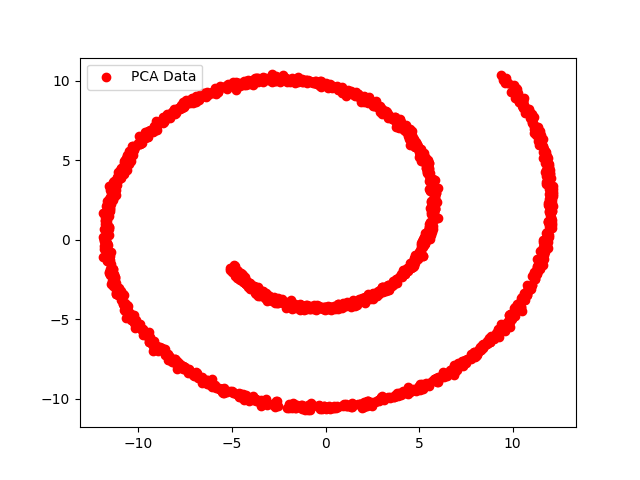
\includegraphics[width=0.7\linewidth]{images/ml_lab4_2.png}
	\caption{}
	\label{fig:mllab42}
\end{figure}

从上图我们可以看出,正投影后得到的形状是信息量最大的方向,于是我们得到了漩涡状的二维图形。

\subsection{人脸数据测试}

我们选取了三幅图片进行测试,分别将降维后的维度设为$(30, 20, 10, 5, 4, 3, 2, 1)$,结果如图\figref{fig:mllab43}、\figref{fig:mllab44}、\figref{fig:mllab45}所示。

\begin{figure}[H]
	\centering
	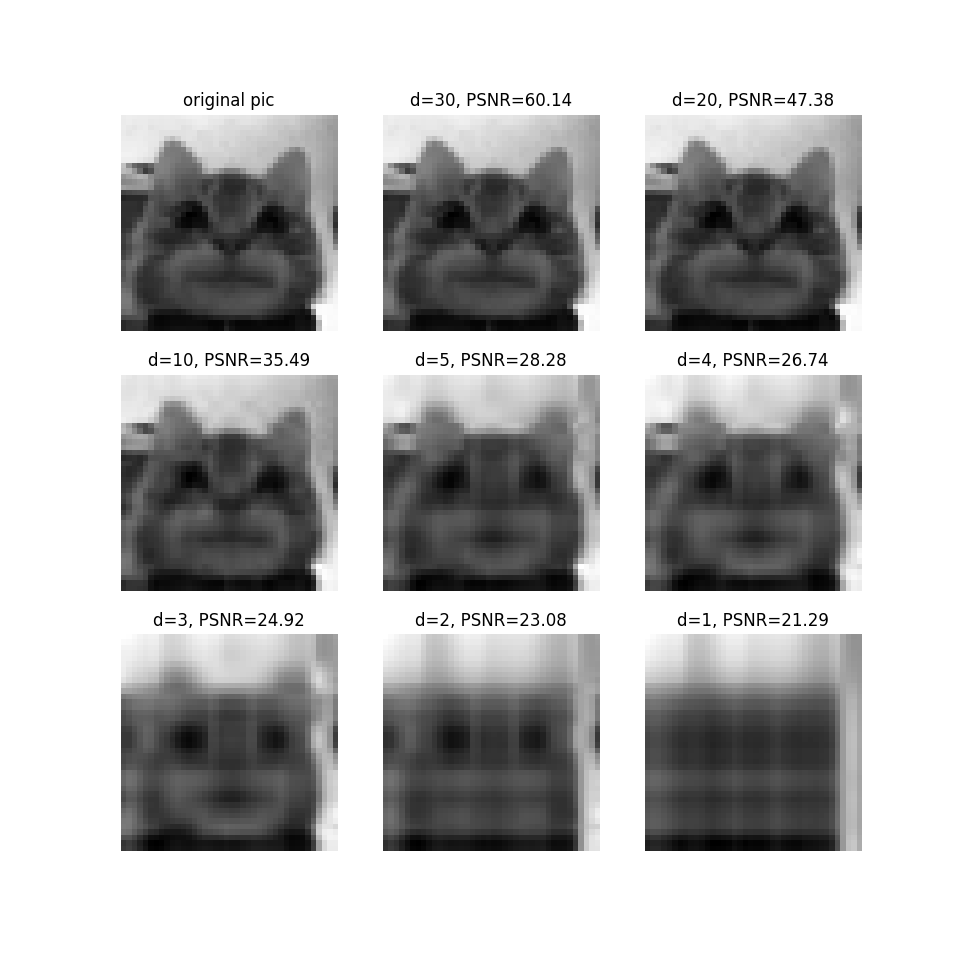
\includegraphics[width=0.6\linewidth]{images/ml_lab4_3.png}
	\caption{}
	\label{fig:mllab43}
\end{figure}

\begin{figure}[H]
	\centering
	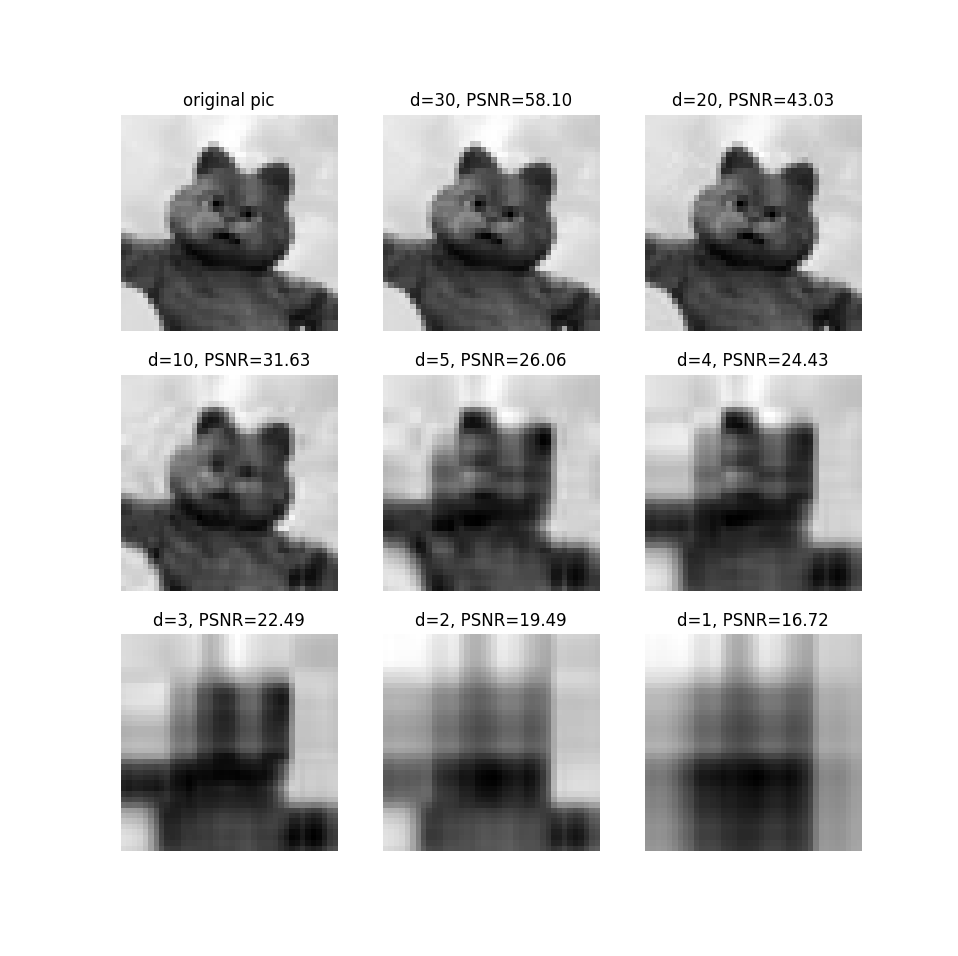
\includegraphics[width=0.6\linewidth]{images/ml_lab4_4.png}
	\caption{}
	\label{fig:mllab44}
\end{figure}

\begin{figure}[H]
	\centering
	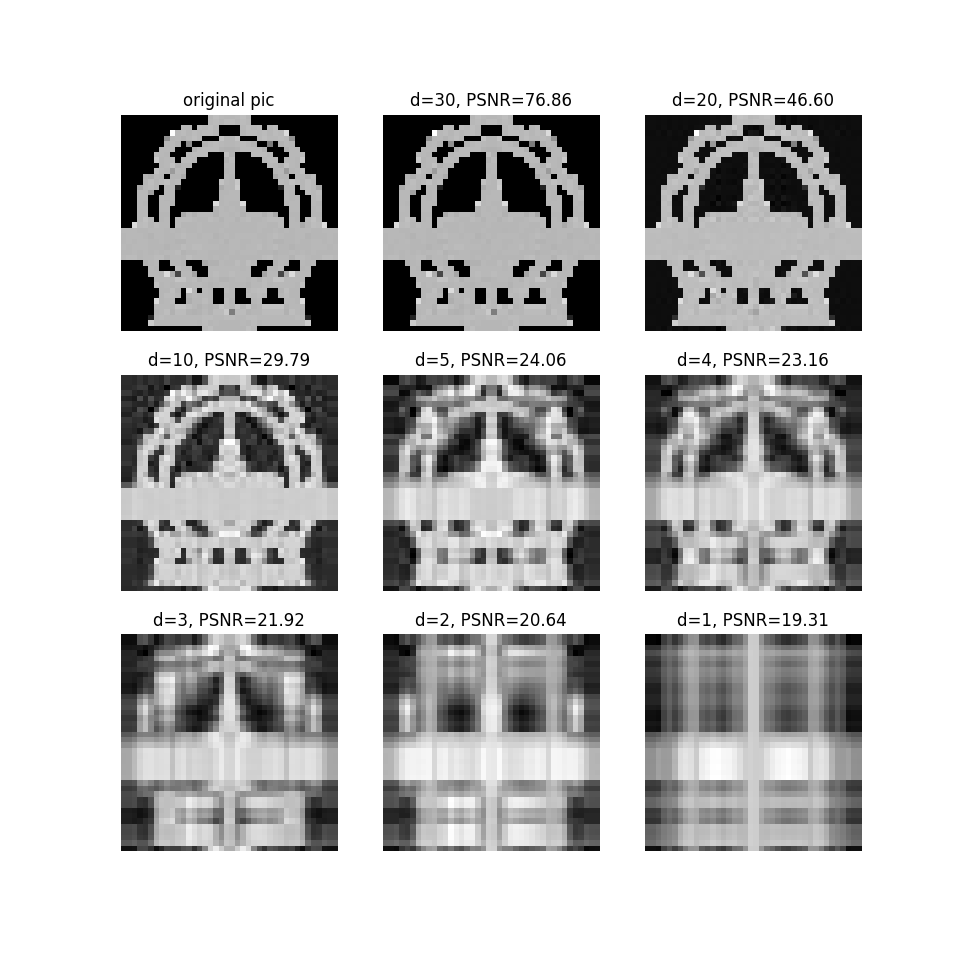
\includegraphics[width=0.6\linewidth]{images/ml_lab4_5.png}
	\caption{}
	\label{fig:mllab45}
\end{figure}

可以看出,在目标维度不小于$20$时,能够较好地保留图片特征,人眼几乎无法分辨损失;目标维度为$5$时,已经能够看出图片明显地损失;当目标维度降到$2$甚至$1$时,已经无法分辨出原来的图像。同时,信噪比随着目标维度的下降而下降。

\section{结论}

PCA在降低数据的维度的同时,保留了主要信息,能够有效地应用于数据压缩、数据降维和图片特征提取等领域。但目标维度的选择对于PCA来说至关重要,需要仔细考虑,太高会使得压缩效果不显著,太低则会导致信息被过度压缩,丢失重要信息。

\nocite{*}

\appendix
%\appendixpage
\addappheadtotoc
\section{源代码(带注释)}
\subsection{生成数据}

\lstinputlisting[
style       =   Python,
caption     =   {\bf data.py},
label       =   {data.py}
]{codes/data.py}


\subsection{PCA}

\lstinputlisting[
style       =   Python,
caption     =   {\bf pca.py},
label       =   {pca.py}
]{codes/pca.py}


\subsection{辅助代码}

\lstinputlisting[
style       =   Python,
caption     =   {\bf utils.py},
label       =   {utils.py}
]{codes/utils.py}


\end{document}
